\documentclass[tikz,border=2pt]{standalone}
\usepackage{amsmath}
\usetikzlibrary{arrows.meta,decorations.pathreplacing}
\begin{document}
% x_{t+3} = 6x_{t+2} - 11x_{t+1} + 6x_t with x_0 = 0, x_1 = 1, x_2 = 5 (so x_t = 3^t - 2^t):
% the state y_0 = (x_0,x_1,x_2) is a window of three values; y_1 = C y_0 shifts the window one step,
% keeping x_1, x_2 and adding x_3 = 19 from the last row of the companion matrix C.
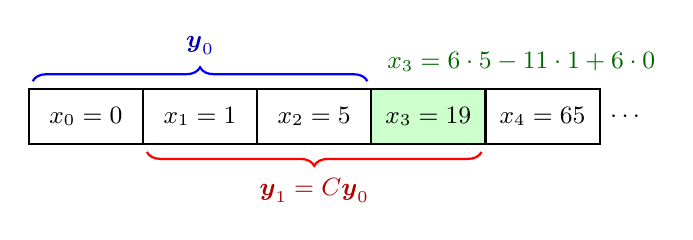
\begin{tikzpicture}[font=\small, >={Latex[length=2mm]}]
  \def\w{1.45}
  \fill[green!20] (3*\w,0) rectangle (4*\w,0.7);
  \foreach \i/\v in {0/0,1/1,2/5,3/19,4/65} {
    \draw[thick] (\i*\w,0) rectangle (\i*\w+\w,0.7);
    \node at (\i*\w+0.5*\w,0.35) {$x_{\i}=\v$};
  }
  \node at (5*\w+0.35,0.35) {$\cdots$};
  % window y_0 above, y_1 below
  \draw[decorate, decoration={brace, amplitude=5pt}, blue, thick] (0.05,0.8) -- (3*\w-0.05,0.8)
    node[midway, above=6pt, blue!70!black] {$\boldsymbol{y}_0$};
  \draw[decorate, decoration={brace, mirror, amplitude=5pt}, red, thick] (\w+0.05,-0.1) -- (4*\w-0.05,-0.1)
    node[midway, below=6pt, red!70!black] {$\boldsymbol{y}_1=C\boldsymbol{y}_0$};
  % new entry from the last row of C
  \node[green!40!black, anchor=south west] at (3*\w+0.08,0.8) {$x_3=6\cdot5-11\cdot1+6\cdot0$};
\end{tikzpicture}
\end{document}
